\documentclass[a4paper, 12pt]{article}
\usepackage[brazilian]{babel} %pacote babel para tweaks em relaçao à linguagem
\usepackage{amsmath}
\usepackage[utf8]{inputenc} %acentos e carácteres específicos
\usepackage[scaled]{helvet}
\renewcommand\familydefault{\sfdefault}
\usepackage[T1]{fontenc}
\usepackage{csquotes} %csquotes auxilia babel
\usepackage[
bottom=2cm,
top=3cm,
left=3cm,
right=2cm,
]{geometry}  %geometry para definição das margens
\usepackage{indentfirst} %primeiro parágrafo "indentado"
\usepackage{tkz-graph} %tkz-graph para criação de grafos
\usepackage{multicol}%para várias colunas
\usepackage{graphicx}

\begin{document}
\title{\textbf{Teoria dos Grafos}\\ \small{Grafos: Tipos, matrizes e graus de um grafo.}}
\author{Leon Ferreira Bellini\\
	\small{\textbf{RA\@ 22218002--8}}\\
	e\\
   Guilherme Ormond Sampaio\\
   \small{\textbf{RA\@ 22218007--7}}
}
\date{}
\maketitle
\section{Introdução}
Um grafo representa de forma simples e eficaz as interdependências entre os elementos de um conjunto. A utilidade da aplicação de grafos tem se mostrado presente em variadas micro e macroestruturas, como a podendo representar cidades, linhas ferroviárias, fluxo de dados ou até mesmo circuitos eletrônicos. A forma de como é representado pode ser dita como didática e facilmente compreendida. Foi elaborado um algoritmo para que fossem aplicados os diversos conceitos aprendidos em aula, este algoritmo sendo desenvolvido em \textbf{Python}, linguagem a qual permite que o programa funcione em variadas plataformas como \textit{GNU/Linux} e \textit{Windows}. 

\begin{center}

	\begin{figure}[hbt]
		\centering
		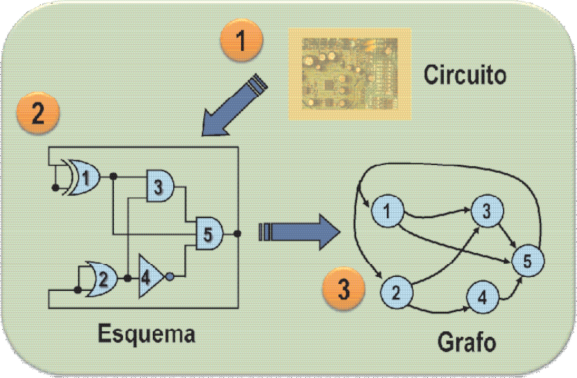
\includegraphics[width=10cm, height= 6cm]{circuito.png}

	\caption[Figura 1]{Circuito eletrônico representado na forma de grafo. -- Grafos: Conceitos, algoritmos e aplicações (2014) }
	\end{figure}

\end{center}

\section{O conceito de grafos}
\subsection{Vértices, arestas e função de incidência {$\varphi$}}
Para que haja um grafo é necessário obter o conjunto de \textbf{vértices}, dado por $\textbf{N} = \{v1, v2, \ldots, vn\}$, estes também chamados de nós, os quais representam os componentes, itens ou elementos que receberão, ou não, ligações entre si, tais ligações chamadas de \textbf{arestas}, as quais também formam um conjunto, dado por $\textbf{E} = \{e1, e2, \ldots, en\}$.

Existe, também, uma \textbf{função de incidência} $ \varphi $ (phi), a qual associa um par de vértices para cada aresta, como por exemplo, $ \varphi(e) = \{ a, b \}$, ou seja, \textit{e} incide em \textit{a} e \textit{b}.

Pode se dizer, então, que um grafo pode ser representado como: \[ G = (N, M, \varphi) \]

	\begin{figure}[hbt]
		\centering
		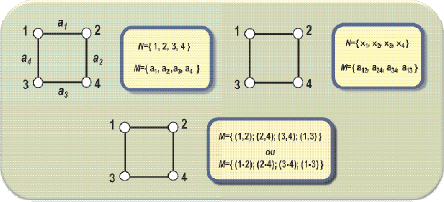
\includegraphics[width=\linewidth]{exemplo.png}

		\caption{Exemplo de como alguns grafos podem ser representados -- Grafos: Conceitos, algoritmos e aplicações (2014) }
	\end{figure}


\subsubsection{Casos Específicos}

\begin{itemize}
	\item\textbf{Grafo Finito}:  \textbf{V} e \textbf{E} são finitos.
	\item\textbf{Grafo Trivial}: Possui apenas um vértice.
	\item\textbf{Grafo Nulo}: Não possui arestas.
\end{itemize}

\pagebreak

\subsubsection{Laços}
    Um laço é uma aresta que possui sua origem e destino em um mesmo vértice, ou seja, incide em um único vértice.
    
    \vspace{0.5in}
    
    Exemplo:
    \begin{figure}[hbt!]
        \begin{center}
            G
            
            \begin{tikzpicture}[scale=1]
                \tikzset{LabelStyle/.style= {fill = white}}
                \Vertex[x=0, y=2]{V1}
                \Vertex[x=2, y=0]{V2}
                \Vertex[x=4, y=3]{V3}
                \Vertex[x=6, y=0]{V4}
                \Edge[label=e1](V1)(V2)
                \Edge[label=e3](V2)(V3)
                \Edge[label=e4](V3)(V4)
                \Edge[label=e5](V4)(V2)
                \Edge[label=e2](V1)(V3)
                \Loop[dist=3cm,dir=WE, style={thick,-}, label=e7](V1)
                \Loop[dist=3cm,dir=EA, style={thick,-}, label=e6](V4)
            \end{tikzpicture}
            \caption{Exemplo de grafo com laços}
        \end{center}
    \end{figure}
    
    \paragraph{}
    As arestas \textbf{e6} e \textbf{e7} são laços.
        
\subsection{Representação matricial de um grafo}

    Para fins de representação não-gráfica dos grafos utiliza-se da matriz de adjacência ou da matriz de incidência.
    
\subsubsection{Matriz de adjacência |A|}

    A matriz de adjacência consiste em uma matriz com \textbf{n}-linhas e \textbf{n}-colunas, sendo \textbf{n} cada vértice do grafo. Os elementos da matriz representam as arestas do grafo, portanto, trata-se da relação de conexões entre seus vértices.
    
    \vspace{0.5in}
    
    \pagebreak
    
    Exemplo:
    
    \begin{figure}[hbt!]
        \begin{multicols}{2}
            \begin{center}
            G\:
            \end{center}
            \begin{tikzpicture}[scale=0.8]
                \Vertex[x=1, y=4]{V1}
                \Vertex[x=4, y=4.5]{V2}
                \Vertex[x=2, y=2.5]{V3}
                \Vertex[x=0, y=2.2]{V4}
                \Vertex[x=3.5, y=0]{V5}
                \Vertex[x=4.2, y=2.3]{V6}
                \Edges(V2,V6,V5,V4,V4,V3,V1)
                \Loop[dist=3cm,dir=WE, style={thick,-}](V4)
                \tikzset{EdgeStyle/.append style = {bend right}}
                \Edge(V2)(V1)
                \tikzset{EdgeStyle/.append style = {bend right}}
                \Edge(V1)(V2)
            \end{tikzpicture}
            
            A (G):
            \begin{tabular}{ccccccc}
                    & V1 & V2 & V3 & V4 & V5 & V6 \\
                    V1 & 0  & 2  & 1  & 0  & 0  & 0  \\
                    V2 & 2  & 0  & 0  & 0  & 0  & 1  \\
                    V3 & 1  & 0  & 0  & 1  & 0  & 0  \\
                    V4 & 0  & 0  & 1  & 1  & 1  & 0  \\
                    V5 & 0  & 0  & 0  & 1  & 0  & 1  \\
                    V6 & 0  & 1  & 0  & 0  & 1  & 0 
            \end{tabular}
        \end{multicols}
        \caption{Exemplo de matriz de adjacência}
    \end{figure}
    
    \vspace{0.5in}
    
    Sendo o elemento \textbf{aij} o número de arestas entre a linha \textbf{Vi} e a coluna \textbf{Vj}. 
    
    \indent Note que por os elementos das linha e colunas se repetirem ocorre um espelhamento diagonal das arestas, ou seja, para a análise do grafo basta observar uma de suas metades. 

    \indent \textbf{obs:} O algoritmo de análise de grafos trabalha a partir dessa matriz.
    
\subsubsection{Matriz de incidência |M|}

    A matriz de adjacência \textbf{M (G) } é uma matriz com \textbf{|V|} linhas e \textbf{|E|} colunas, tal que seus elementos (\textbf{aij}) representam quantas vezes a aresta \textbf{ej} incide no vértice \textbf{Vi}.
    
    \vspace{0.5in}
    
    Exemplo:
    
    \begin{figure}[hbt!]
        \begin{multicols}{2}
            \begin{center}
            G\:
            \end{center}
            \begin{tikzpicture}[scale=1]
                \tikzset{LabelStyle/.style= {fill = white}}
                \Vertex[x=1, y=4]{V1}
                \Vertex[x=4, y=4.5]{V2}
                \Vertex[x=2, y=2.5]{V3}
                \Vertex[x=0, y=2.2]{V4}
                \Vertex[x=3.5, y=0]{V5}
                \Vertex[x=4.2, y=2.3]{V6}
                \Edge[label=e3](V1)(V3)
                \Edge[label=e4](V3)(V4)
                \Edge[label=e6](V4)(V5)
                \Edge[label=e7](V5)(V6)
                \Edge[label=e8](V6)(V2)
                \Loop[dist=3cm,dir=WE, style={thick,-}, label=e5](V4)
                \tikzset{EdgeStyle/.append style = {bend right}}
                \Edge[label=e1](V2)(V1)
                \tikzset{EdgeStyle/.append style = {bend right}}
                \Edge[label=e2](V1)(V2)
            \end{tikzpicture}
            
            \begin{center}
            M (G):
            \end{center}
            \begin{tabular}{ccccccccc}
                & e1 & e2 & e3 & e4 & e5 & e6 & e7 & e8 \\
                V1 & 1  & 1  & 1  & 0  & 0  & 0  & 0  & 0  \\
                V2 & 1  & 1  & 0  & 0  & 0  & 0  & 0  & 1  \\
                V3 & 0  & 0  & 1  & 1  & 0  & 0  & 0  & 0  \\
                V4 & 0  & 0  & 0  & 1  & 2  & 1  & 0  & 0  \\
                V5 & 0  & 0  & 0  & 0  & 0  & 1  & 1  & 0  \\
                V6 & 0  & 0  & 0  & 0  & 0  & 0  & 1  & 1 
            \end{tabular}
        \end{multicols}
        \caption{Exemplo de matriz de incidência}
    \end{figure}
    
    \vspace{0.5in}
    
    Note que, por uma aresta estar conectada sempre em dois pontos, a soma dos elementos de cada coluna é 2.
    
\subsection{Grafo simples}

Um grafo é simples se não possui laços ou arestas múltiplas, logo, tendo-se como exemplo um grafo \textbf{G} possuindo $\textbf{V} = \{v1, v2, v3, v4\}$ e $\textbf{E} = \{e1, e2, e3, e4, e5\}$, sua matriz de adjacência \textbf{A} pode ser dada por:
 

\begin{figure}[hbt!]
	
    \begin{multicols}{2}
	    \centering
	    G
	    \[
        \begin{tikzpicture}[scale=1]
            \Vertex[x=1, y=4]{V1}
            \Vertex[x=4, y=4]{V2}
            \Vertex[x=4, y=1]{V3}
            \Vertex[x=1, y=1]{V4}
	    \Edges(V1,V2,V2,V3,V3,V4,V4,V1,V4,V2,V1,V3)
        \end{tikzpicture}
\]
\[
	A(G) = 
\begin{bmatrix}
	0	&1	&1 	&1 \\
	1	&0	&1	&1 \\
	1	&1	&0	&1  \\
	1	&1	&1	&0
\end{bmatrix} \]

\end{multicols}
\caption{Exemplo de grafo \textbf{G} e matriz de adjacência \textbf{A (G)} simples}
\end{figure}
\textbf{obs}: Note que a diagonal principal da matriz indica se existem ou não, laços. Um número maior que 1 indicaria que existem mais de uma aresta ligando os dois vértices. Podem existir vértices de grau 0 em grafos simples.

\subsubsection{Grafo bipartido}
É um tipo de grafo simples o qual, uma vez que seus vértices são divididos em subconjuntos \textbf{X} e \textbf{Y}, possui cada aresta com uma de suas pontas no conjunto \textbf{X} e outra em \textbf{Y}.


\begin{center}
	G\:
	\begin{figure}[hbt!]
		\centering
        \begin{tikzpicture}[scale=1]
            \Vertex[x=1, y=4]{V1}
            \Vertex[x=4, y=4]{V2}
            \Vertex[x=4, y=1]{V3}
            \Vertex[x=1, y=1]{V4}
	    \Edges(V1,V2, V1,V4,V3,V4, V3,V2)

        \end{tikzpicture}
	  \caption{$X = \{V1, V2\}$ $Y = \{V3, V4\}$}
\end{figure}
\end{center}\hspace{1cm}

Um grafo é dado por \textbf{Bipartido completo} quando cada vértice em X é adjacente a todo vértice em Y. É escrito através da letra $\textbf{K}{mn}$, sendo |x| = m e |y| = n.

\pagebreak

\begin{center}
	G\:
	\begin{figure}[hbt!]
		\centering
        \begin{tikzpicture}[scale=1]
            \Vertex[x=2, y=4]{V1}
            \Vertex[x=4, y=4]{V2}
            \Vertex[x=6, y=1]{V3}
            \Vertex[x=3, y=1]{V4}
	    \Vertex[x=0, y=1]{V5}
	    \Edges(V1,V5, V1,V4, V1,V3, V2,V5, V2,V4, V2, V3)
        \end{tikzpicture}

	\caption{$X = \{V1, V2\}$ $Y = \{V3, V4, V5\}$}
\end{figure}
\end{center}


\subsection{Graus de um vértice}

    Cada vértice \textbf{V} de um grafo \textbf{G = (V, E)} possui um número \textbf{n} de arestas incidentes. Esse número \textbf{n} é denotado como o grau do vértice.
    
    \begin{figure}[hbt!]
        \begin{multicols}{2}
            \begin{center}
            G
            \end{center}
            \begin{tikzpicture}[scale=1]
                \tikzset{LabelStyle/.style= {fill = white}}
                \Vertex[x=4, y=6]{V1}
                \Vertex[x=0, y=3]{V2}
                \Vertex[x=4, y=3]{V3}
                \Vertex[x=0, y=0]{V4}
                \Vertex[x=4, y=0]{V5}
                \Edge[label=e1](V1)(V2)
                \Edge[label=e2](V1)(V3)
                \Edge[label=e3](V3)(V5)
                \Edge[label=e4](V5)(V4)
                \Edge[label=e5](V4)(V2)
                \Edge[label=e6](V2)(V5)
                \Loop[dist=3cm,dir=WE, style={thick,-}, label=e7](V2)
            \end{tikzpicture}
        
            A (G):
            \begin{tabular}{cccccc}
                & V1 & V2 & V3 & V4 & V5 \\
                V1 & 0  & 1  & 1  & 0  & 0  \\
                V2 & 1  & 1  & 0  & 1  & 1  \\
                V3 & 1  & 0  & 0  & 0  & 1  \\
                V4 & 0  & 1  & 0  & 0  & 1  \\
                V5 & 0  & 1  & 1  & 1  & 0 
            \end{tabular}
            
            \vspace{0.4in}
            Graus:
            \begin{tabular}{cc}
                & Grau \\
                V1 & 2    \\
                V2 & 5    \\
                V3 & 2    \\
                V4 & 2    \\
                V5 & 3   
            \end{tabular}
        \end{multicols}
        \caption{Grafo \textbf{G}, matriz de adjacência \textbf{A (G)} e tabela de graus dos vértices do grafo \textbf{G}}
    \end{figure}
    
    Note que os laços incidem duas vezes no vértice, portanto ele equivale a 2 graus, como o caso da aresta \textbf{e7}.
    
    \indent Para calcular o grau em uma matriz adjacência basta somar todos os elementos da linha ou coluna ignorando o elemento da diagonal principal + 2 * o elemento da diagonal principal, que indica os laços.
    
\subsection{Sequência gráfica}

    A sequência de graus de um grafo \textbf{G = (V, E)} é a sequência não-crescente do grau de todos os vértices \textbf{V} desse grafo. 
    
    \indent Para o caso da figura 9 a sequência seria:
    
    \begin{center}
     5, 3, 2, 2, 2
    \end{center}

\section{Resultados}

O algoritmo ou \textit{script} mostrou-se eficaz ao tratar e testar as mais diversas matrizes de adjacência inseridas. Este, porém, não realizando testes quanto à legitimidade dos dados, confiando totalmente no usuário. Foram realizados 10 testes com grafos contendo variadas quantidades de vértices.

Para elaboração do programa e teoria aplicada nesse relatório, foram utilizados como referência o material providenciado pelo professor, além do item de bibliografia básica ``Grafos: Conceitos, algoritmos e aplicações''. 

\begin{figure}[hbt!]
\begin{multicols}{2}
	\[
	\begin{bmatrix}
	0	&0	&1 	&1	&1\\
	0	&0	&1	&1 	&1\\
	1	&1	&0	&1  	&1\\
	1	&1	&1	&0	&1\\
	1	&1	&1	&1	&0

\end{bmatrix} \]

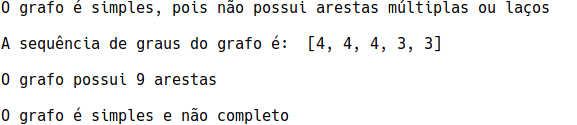
\includegraphics[width=\linewidth]{outputprog.png}
\end{multicols}
\caption{Matriz de adjacência genérica para teste de grafos simples e o respectivo \textit{output}. }
\end{figure}
\section{Conclusão}

    A partir da elaboração do algoritmo é possível observar a dependência entre os conceitos de grafos e a obrigatoriedade de um conhecimento prévio para este caso de algoritmo genérico, uma vez que suas respostas são também genéricas e possuem significados distintos dependendo da aplicação. 
    
    \indent É possível observar ainda a utilidade da representação matricial, visto que um grafo dotado de excessiva complexidade se torna penoso para ser analisado graficamente. A matriz permite a automatização desse processo, que é repetitivo e padronizado.
    
    \indent Apesar da praticidade proporcionada pelo algoritmo, uma representação matricial não deve ser dita como a representação precisa de um grafo. Um grafo possui uma única posição relativa, no qual não é considerada em uma matriz, ou seja, a representação matricial pode ser escrita a partir de uma representação gráfica, mas não o oposto.

\section{Referências bibliográficas}
GOLDBARG, Marco e Elizabeth. \textbf{Grafos: Conceitos, algoritmos e aplicações.}1.ed.- São Paulo: Elsevier,2012.
\end{document}
